\chapter{Conception logicielle}
\addcontentsline{toc}{chapter}{Conception logicielle}

\section{Architecture logicielle}
L’application suit une architecture modulaire basée sur le MVVM(modèle-vue-vue modèle), divisée en trois couches principales :

\begin{itemize}
\item    Présentation (UI) : Gérée par des Composants Jetpack Compose et des ViewModels.
\item    Domain (Métier) : Contient les Use Cases et les interfaces de Repository.
\item    Data (Accès aux données) : Implémente les sources de données (Firebase, ESP32, Capteurs).
\end{itemize}
Pour des soucis de performance, les données envoyés aux microcontrôleurs sont des données de types booléennes, pour que l'éxecution se fait approximativement en temps réel. 


\section{Structure de la base de données dans Realtime Database}

L'application utilise une base de données de type \textit{clé-valeur} appelée \textbf{Realtime Database}, hébergée et gérée par Firebase. Cette base de données offre plusieurs avantages, tels qu'une infrastructure sans serveur, une haute disponibilité et une sécurité assurée par Google. La structure des données utilisée est illustrée à la figure~\ref{fig:structure_de_la_base_de_donnees}.

\begin{figure}[H]
   \centering
   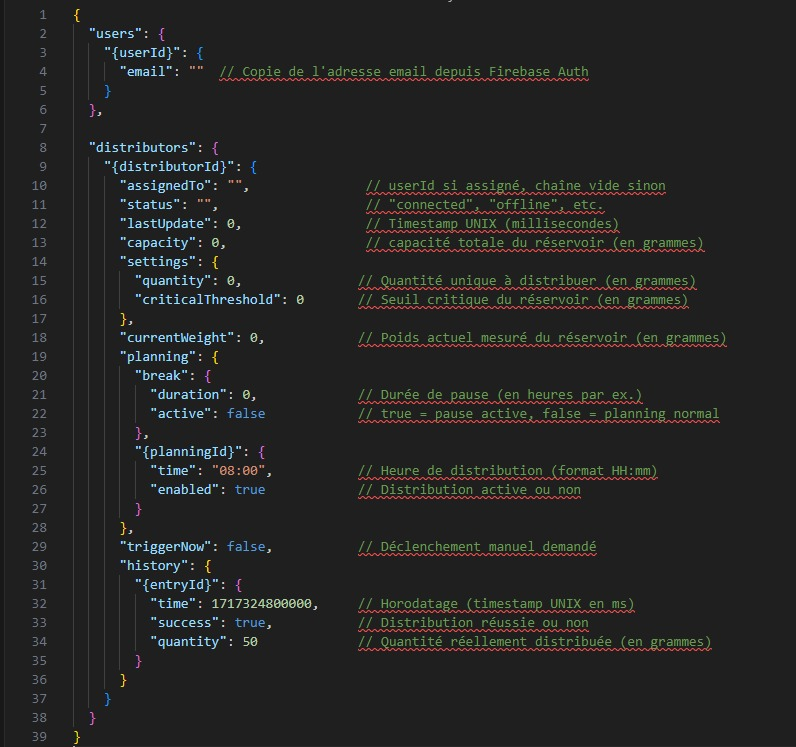
\includegraphics[scale=0.5]{dd3.jpeg}
   \caption{Structure de la base de données}
   \label{fig:structure_de_la_base_de_donnees}
\end{figure}

La base de données contient deux clés principales :

\begin{itemize}
\item \textbf{users} : contient les informations de tous les utilisateurs de l'application mobile.
\item \textbf{distributors} : contient les paramètres des distributeurs automatiques de nourriture pour chats.
\end{itemize}

\begin{enumerate}[label=\alph*)]
\item \textbf{Données des utilisateurs} 

\textbf{Firebase Authentication} est utilisé pour gérer l'authentification des utilisateurs. Les informations d'authentification sont stockées et gérées par ce service. Les données spécifiques à chaque utilisateur, stockées dans Realtime Database, sont :

\begin{itemize}
\item \textbf{\{userId\}} : identifiant unique généré par Firebase Authentication pour chaque utilisateur.
\item \textbf{email} : adresse e-mail utilisée par l'utilisateur pour se connecter à l'application.
\end{itemize}

\item{Données des distributeurs} 

Les données des distributeurs servent principalement à configurer leurs actions. Ces données incluent :

\begin{itemize}
\item \textbf{\{distributorId\}} : identifiant unique de chaque distributeur, généré lors de l'assemblage du matériel.
\item \textbf{assignedTo} : identifiant de l'utilisateur associé au distributeur.
\item \textbf{status} : état de la connexion Internet de l'ESP32.
\item \textbf{lastUpdate} : date de la dernière activité du distributeur.
\item \textbf{capacity} : capacité totale du réservoir en grammes.
\item \textbf{settings} : paramètres de distribution des croquettes, comprenant :
  \begin{itemize}
    \item \textit{quantity} : quantité à distribuer en grammes.
    \item \textit{criticalThreshold} : seuil critique du réservoir en grammes.
  \end{itemize}
\item \textbf{currentWeight} : poids actuel mesuré du réservoir en grammes.
\item \textbf{planning} : liste des distributions programmées par l'utilisateur. Chaque entrée contient :
  \begin{itemize}
    \item \textit{time} : heure de distribution au format \textit{HH:mm}.
    \item \textit{enabled} : indique si la distribution est active.
    \item \textit{break} : indique une pause dans la distribution.
  \end{itemize}
\item \textbf{triggerNow} : booléen indiquant un déclenchement manuel du distributeur.
\item \textbf{history} : historique des distributions effectuées.
\end{itemize}



\end{enumerate}

\section{Fonctionalité clés de l’application} 

\subsection{Gestion des utilisateurs (Firebase Auth)}
L'inscription et la connexion se fait via email et mot de passe. Seul l’utilisateur authentifié peut contrôler son distributeur.

\subsection{Programmation des repas} 
Les horaires de distributions et la quantité sont stockés dans Firebase avec \textbf{Real Time Database}.

\subsection{Contrôle manuel}
On envoi une commande depuis Firebase qui provoque un déclenchement immédiat sur l’ESP32. Un "trigger" de type booléen qui permet au microcontrôleur d'effectuer  ou non une action sur l'ensemble du système.

\subsection{Notifications}
Des alertes sont envoyés, comme la confirmation de la nourriture distribuée et le niveau de nourriture faible. Ces notifications viennent de l'application mobile, qui envoi un "trigger"



\chapter{Conception électronique}
%\addcontentsline{toc}{chapter}{Conception électronique}



